\documentclass[11pt,compress,t,notes=noshow, xcolor=table]{beamer}
% graphicx and color are loaded via lmu-lecture.sty
% maxwidth is the original width if it is less than linewidth
% otherwise use linewidth (to make sure the graphics do not exceed the margin)
% TODO: Remove once cleared to be superfluous
% \makeatletter
% \def\maxwidth{ %
%   \ifdim\Gin@nat@width>\linewidth
%     \linewidth
%   \else
%     \Gin@nat@width
%   \fi
% }
% \makeatother

% ---------------------------------%
% latex-math dependencies, do not remove:
% - mathtools
% - bm
% - siunitx
% - dsfont
% - xspace
% ---------------------------------%

%--------------------------------------------------------%
%       Language, encoding, typography
%--------------------------------------------------------%

\usepackage[english]{babel}
\usepackage[utf8]{inputenc} % Enables inputting UTF-8 symbols
% Standard AMS suite (loaded via lmu-lecture.sty)

% Font for double-stroke / blackboard letters for sets of numbers (N, R, ...)
% Distribution name is "doublestroke"
% According to https://mirror.physik.tu-berlin.de/pub/CTAN/fonts/doublestroke/dsdoc.pdf
% the "bbm" package does a similar thing and may be superfluous.
% Required for latex-math
\usepackage{dsfont}

% bbm – "Blackboard-style" cm fonts (https://www.ctan.org/pkg/bbm)
% Used to be in common.tex, loaded directly after this file
% Maybe superfluous given dsfont is loaded
% TODO: Check if really unused?
% \usepackage{bbm}

% bm – Access bold symbols in maths mode - https://ctan.org/pkg/bm
% Required for latex-math, preferred over \boldsymbol
% https://tex.stackexchange.com/questions/3238/bm-package-versus-boldsymbol
\usepackage{bm}

% pifont – Access to PostScript standard Symbol and Dingbats fonts
% Used for \newcommand{\xmark}{\ding{55}, which is never used
% aside from lecture_advml/attic/xx-automl/slides.Rnw
% \usepackage{pifont}

% Quotes (inline and display), provdes \enquote
% https://ctan.org/pkg/csquotes
\usepackage{csquotes}

% Adds arg to enumerate env, technically superseded by enumitem according
% to https://ctan.org/pkg/enumerate
% Replace with https://ctan.org/pkg/enumitem ?
% Even better: enumitem is not really compatible with beamer and breaks all sorts of things
% particularly the enumerate environment. The enumerate package also just isn't required
% from what I can tell so... don't re-add it I guess?
% \usepackage{enumerate}

% Line spacing - provides \singlespacing \doublespacing \onehalfspacing
% https://ctan.org/pkg/setspace
% \usepackage{setspace}

% mathtools – Mathematical tools to use with amsmath
% https://ctan.org/pkg/mathtools?lang=en
% latex-math dependency according to latex-math repo
\usepackage{mathtools}

% Maybe not great to use this https://tex.stackexchange.com/a/197/19093
% Use align instead -- TODO: Global search & replace to check, eqnarray is used a lot
% $ rg -f -u "\begin{eqnarray" -l | grep -v attic | awk -F '/' '{print $1}' | sort | uniq -c
%   13 lecture_advml
%   14 lecture_i2ml
%    2 lecture_iml
%   27 lecture_optimization
%   45 lecture_sl
\usepackage{eqnarray}
% For shaded regions / boxes
% Used sometimes in optim
% https://www.ctan.org/pkg/framed
\usepackage{framed}

%--------------------------------------------------------%
%       Cite button (version 2024-05)
%--------------------------------------------------------%

% Superseded by style/ref-buttons.sty, kept just in case these don't work out somehow.

% Note this requires biber to be in $PATH when running,
% telltale error in log would be e.g. Package biblatex Info: ... file 'authoryear.dbx' not found
% aside from obvious "biber: command not found" or similar.
% Tried moving this to lmu-lecture.sty but had issues I didn't quite understood,
% so it's here for now.

\usepackage{hyperref}

% Only try adding a references file if it exists, otherwise
% this would compile error when references.bib is not found
% NOTE: Bibliography packages (usebib, biblatex) are now loaded by ref-buttons.sty when needed
% This keeps all bibliography-related setup in one place

% Legacy \citelink command removed - superseded by ref-buttons.sty

%--------------------------------------------------------%
%       Displaying code and algorithms
%--------------------------------------------------------%

% Reimplements verbatim environments: https://ctan.org/pkg/verbatim
% verbatim used sed at least once in
% supervised-classification/slides-classification-tasks.tex
% Removed since code should not be put on slides anyway
% \usepackage{verbatim}

% Both used together for algorithm typesetting, see also overleaf: https://www.overleaf.com/learn/latex/Algorithms
% algorithmic env is also used, but part of the bundle:
%   "algpseudocode is part of the algorithmicx bundle, it gives you an improved version of algorithmic besides providing some other features"
% According to https://tex.stackexchange.com/questions/229355/algorithm-algorithmic-algorithmicx-algorithm2e-algpseudocode-confused
\usepackage{algorithm}
\usepackage{algpseudocode}

%--------------------------------------------------------%
%       Tables
%--------------------------------------------------------%

% multi-row table cells: https://www.namsu.de/Extra/pakete/Multirow.html
% Provides \multirow
% Used e.g. in evaluation/slides-evaluation-measures-classification.tex
\usepackage{multirow}

% colortbl: https://ctan.org/pkg/colortbl
% "The package allows rows and columns to be coloured, and even individual cells." well.
% Provides \columncolor and \rowcolor
% \rowcolor is used multiple times, e.g. in knn/slides-knn.tex
\usepackage{colortbl}

% long/multi-page tables: https://texdoc.org/serve/longtable.pdf/0
% Not used in slides
% \usepackage{longtable}

% pretty table env: https://ctan.org/pkg/booktabs
% Is used
% Defines \toprule
\usepackage{booktabs}

%--------------------------------------------------------%
%       Figures: Creating, placing, verbing
%--------------------------------------------------------%

% wrapfig - Wrapping text around figures https://de.overleaf.com/learn/latex/Wrapping_text_around_figures
% Provides wrapfigure environment -used in lecture_optimization
\usepackage{wrapfig}

% Sub figures in figures and tables
% https://ctan.org/pkg/subfig -- supersedes subfigure package
% Provides \subfigure
% \subfigure not used in slides but slides-tuning-practical.pdf errors without this pkg, error due to \captionsetup undefined
\usepackage{subfig}

% Actually it's pronounced PGF https://en.wikibooks.org/wiki/LaTeX/PGF/TikZ
\usepackage{tikz}

% No idea what/why these settings are what they are but I assume they're there on purpose
\usetikzlibrary{shapes,arrows,automata,positioning,calc,chains,trees, shadows}
\tikzset{
  %Define standard arrow tip
  >=stealth',
  %Define style for boxes
  punkt/.style={
    rectangle,
    rounded corners,
    draw=black, very thick,
    text width=6.5em,
    minimum height=2em,
    text centered},
  % Define arrow style
  pil/.style={
    ->,
    thick,
    shorten <=2pt,
    shorten >=2pt,}
}

%--------------------------------------------------------%
%       Beamer setup and custom macros & environments
%--------------------------------------------------------%

% Main sty file for beamer setup (layout, style, lecture page numbering, etc.)
% For long-term maintenance, this may me refactored into a more modular set of .sty files
\usepackage{../../style/lmu-lecture}
% Custom itemize wrappers, itemizeS, itemizeL, etc
\usepackage{../../style/customitemize}
% Custom framei environment, uses custom itemize!
\usepackage{../../style/framei}
% Custom frame2 environment, allows specifying font size for all content
\usepackage{../../style/frame2}
% Column layout macros
\usepackage{../../style/splitV}
% \image and derivatives
\usepackage{../../style/image}
% New generation of reference button macros
\usepackage{../../style/ref-buttons}

% Used regularly
\let\code=\texttt

% Not sure what/why this does
\setkeys{Gin}{width=0.9\textwidth}

% -- knitr leftovers --
% These may be used by knitr/R Markdown workflows in other lectures
\makeatletter
\def\maxwidth{ %
  \ifdim\Gin@nat@width>\linewidth
    \linewidth
  \else
    \Gin@nat@width
  \fi
}
\makeatother

% Define colors for syntax highlighting (may be used by knitr)
\definecolor{fgcolor}{rgb}{0.345, 0.345, 0.345}
\definecolor{shadecolor}{rgb}{.97, .97, .97}

% knitr code output environment
\newenvironment{knitrout}{}{}


% Can't find a reason why common.tex is not just part of this file?
% This file is included in slides and exercises

% Rarely used fontstyle for R packages, used only in 
% - forests/slides-forests-benchmark.tex
% - exercises/single-exercises/methods_l_1.Rnw
% - slides/cart/attic/slides_extra_trees.Rnw
\newcommand{\pkg}[1]{{\fontseries{b}\selectfont #1}}

% Spacing helpers, used often (mostly in exercises for \dlz)
\newcommand{\lz}{\vspace{0.5cm}} % vertical space (used often in slides)
\newcommand{\dlz}{\vspace{1cm}}  % double vertical space (used often in exercises, never in slides)
\newcommand{\oneliner}[1] % Oneliner for important statements, used e.g. in iml, algods
{\begin{block}{}\begin{center}\begin{Large}#1\end{Large}\end{center}\end{block}}

% Don't know if this is used or needed, remove?
% textcolor that works in mathmode
% https://tex.stackexchange.com/a/261480
% Used e.g. in forests/slides-forests-bagging.tex
% [...] \textcolor{blue}{\tfrac{1}{M}\sum^M_{m} [...]
% \makeatletter
% \renewcommand*{\@textcolor}[3]{%
%   \protect\leavevmode
%   \begingroup
%     \color#1{#2}#3%
%   \endgroup
% }
% \makeatother



\title{Introduction to Machine Learning}

\begin{document}

% Removed figure here on bernd's explicit wish to substitute with something else

\titlemeta{% Chunk title (example: CART, Forests, Boosting, ...), can be empty
  ML-Basics
  }{% Lecture title  
  What is Machine Learning?
}{% Relative path to title page image: Can be empty but must not start with slides/
}{% Learning goals, wrapped inside itemize environment
  \item Understand basic terminology of and connections between ML, AI, DL and statistics
  \item Know the main directions of ML: Supervised, Unsupervised and Reinforcement Learning
}

% ------------------------------------------------------------------------------

\begin{frame}{Machine Learning is changing our world}

\begin{itemize}

  \item Search engines learn what you want
  
  \item Recommender systems learn your taste in books, music, movies,...
  
  \item Algorithms do automatic stock trading
  
  \item Google Translate learns how to translate text
  
  \item Siri learns to understand speech
  
  \item DeepMind beats humans at Go
  
  \item Cars drive themselves
  
  % \item Medicines are developed faster
  
  \item Smart-watches monitor your health
  
  \item Election campaigns use algorithmically targeted ads to influence voters
  
  \item Data-driven discoveries are made in physics, biology, genetics, 
  astronomy, chemistry, neurology,...
  
  \item ...
  
\end{itemize}

\end{frame}

% ------------------------------------------------------------------------------

\begin{frame}{The World of Artificial Intelligence}

... and the connections to Machine Learning and Deep Learning

% Machine learning is a branch of statistics and computer science. 

\begin{center}

  \begin{figure}
    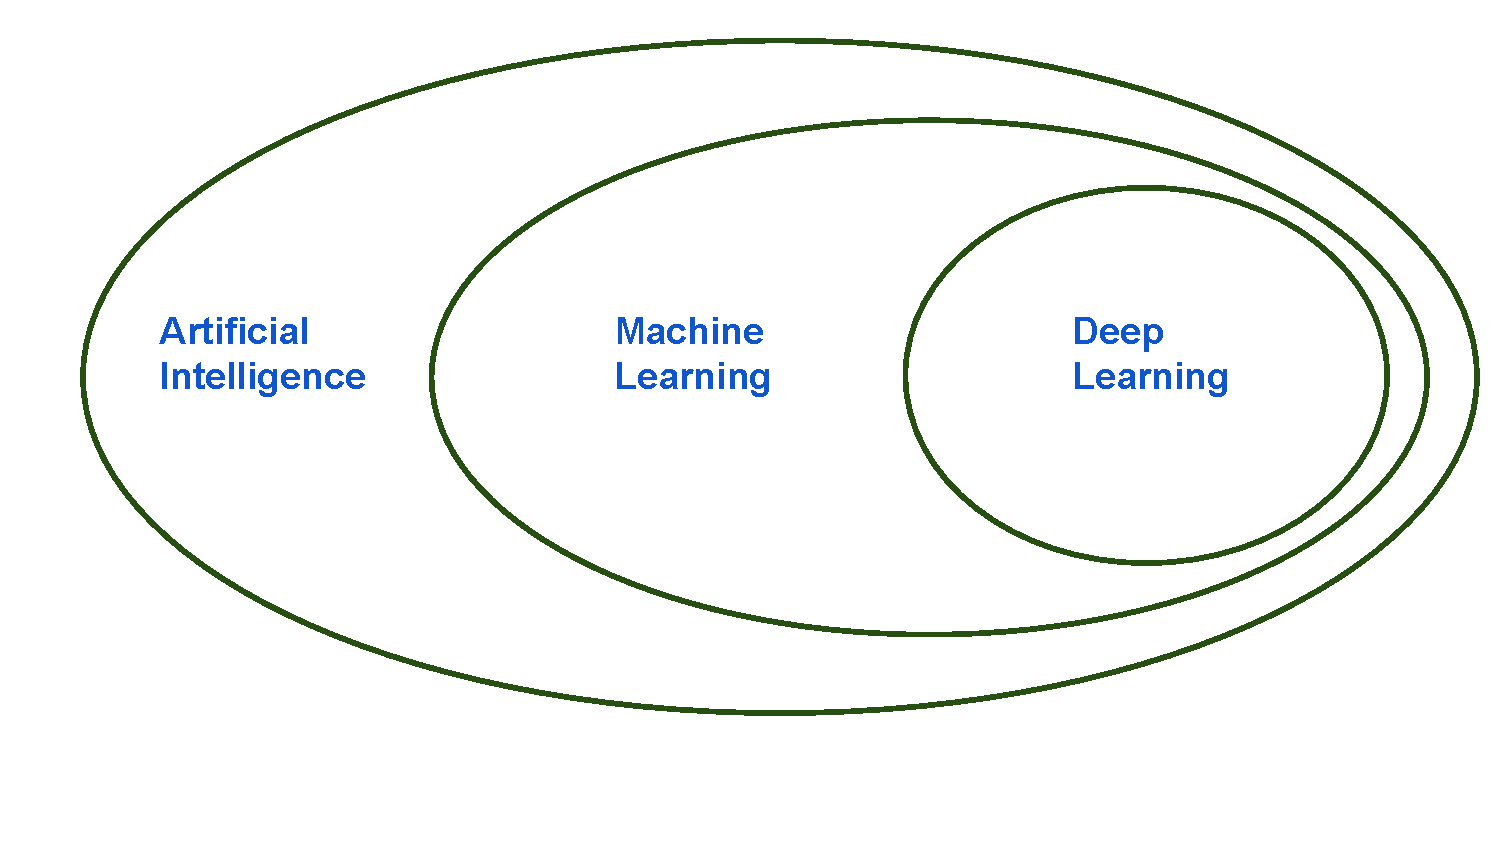
\includegraphics[width=0.7\textwidth]{figure_man/learning} 
  \end{figure}

  \lz

Many people are confused what these terms actually mean. 

\lz

And what does all this have to do with statistics?

  % Machine Learning is a method of teaching computers to make predictions based 
  % on some data.

%  A computer program is said to \textbf{learn} from experience E with respect to
%  some task T and some performance measure P, if its performance on T, as 
%  measured by P, improves with experience E. \\
%  
%  \begin{footnotesize}
%  \emph{Tom Mitchell, Carnegie Mellon University, 1998}
%  \end{footnotesize}
  
  \end{center}
  
\end{frame}

% ------------------------------------------------------------------------------

\begin{frame}{Artificial Intelligence}

\begin{itemize}
	\item AI is a general term for a very large and rapidly developing field.
	\item There is no strict definition of AI, but it's often used when machines are trained to perform on tasks which until that time could only be solved by humans or are very difficult and assumed to require "intelligence".
    \item AI started in the 1940s - when the computer was invented. Scientists like 
        Turing and John von Neumann immediately asked the question:
        If we can formalize computation, can we use computation to formalize "thinking"?
	\item AI includes machine learning, natural language processing, computer vision, robotics, planning, search, game playing, intelligent agents, and much more.
    \item Nowadays, AI is a "hype" term that many people use when they should probably say: ML or ... basic data analysis.
\end{itemize}
  
\end{frame}

% ------------------------------------------------------------------------------

\begin{frame}{Machine Learning}

\begin{columns}
\begin{column}{0.65\textwidth}
\begin{center}
  % FIGURE SOURCE: https://www.oreilly.com/library/view/java-deep-learning/9781788997454/assets/899ceaf3-c710-4675-ae99-33c76cd6ac2f.png
  % \includegraphics[width=0.7\textwidth]{figure_man/l}
  \includegraphics[trim=0 0 0 0,clip,width=\textwidth]{figure_man/whatisml.png}\\[3ex]
  \tiny{Image via \url{https://www.oreilly.com/library/view/java-deep-learning/9781788997454/assets/899ceaf3-c710-4675-ae99-33c76cd6ac2f.png}}
\end{center}
\end{column}
\begin{column}{0.45\textwidth}
\begin{footnotesize}
\begin{itemize}
    % \item Mainly includes supervised, unsup. and reinforcement learning.
	\item Mathematically well-defined and solves reasonably narrow tasks.
	\item ML algorithms usually construct predictive/decision models from data, instead of explicitly programming them.
    \item A computer program is said to learn from experience E with respect to
  some task T and some performance measure P, if its performance on T, as 
  measured by P, improves with experience E. \\
  \begin{footnotesize}
  \emph{Tom Mitchell, Carnegie Mellon University, 1998}
  \end{footnotesize}
\end{itemize}
\end{footnotesize}
\end{column}
\end{columns}
  
\end{frame}

\begin{vbframe}{Deep Learning}

\begin{itemize}
\item DL is a subfield of ML which studies neural networks.
\item Artificial neural networks (ANNs) might have been (roughly) inspired by the human brain, but they are simply a certain model class of ML.
\item ANNs have been studied for decades. DL uses more layers, 
        specific neurons were invented for images and tensors and many computational 
        improvements allow training on large data.
	% \item The term refers to the fact that rather complex neural networks, i.e. \emph{deep} networks are used
\item DL can be used on tabular data, but typical applications are images, texts or signals. 
\item The last 10-15 years have produced remarkable results and imitations of human ability, where the result looked intelligent. 
\end{itemize}

\lz

"Any sufficiently advanced technology is indistinguishable from magic."
\begin{footnotesize}
\emph{Arthur C. Clarke's 3rd law}
\end{footnotesize}
 

\end{vbframe}

% ------------------------------------------------------------------------------

\begin{frame}{ML vs. Stats}


\begin{itemize}
	\item ML and Statistics have historically been developed in different fields, but many
      methods and especially the mathematical foundations are equivalent.
	\item Traditionally, models from ML focused more on precise predictions whereas models from statistics focused more on the ability to interpret the patterns that generated the data and the ability to derive sound inference.
	\item Nowadays, ML and predictive modelling in statistics basically work on the same problems with the same tools.
    \item Unfortunately, the communities are still divided, don't talk to each other as much as they should and everyone is confused due to different terminology for the same concepts.
        % from both worlds can be used for similar tasks because ML models have gained in interpretability and statistics models have gained in predictive power
    \item Most parts of ML we could also call:\\Nonparametric statistics plus efficient numerical optimization.
\end{itemize}

\end{frame}


\begin{vbframe}{Unsupervised learning}
\begin{itemize}
  \item Data without labels $y$
  \item Search for patterns within the inputs $x$
  \item \textit{Unsupervised} as there is no \enquote{true} output
      we can optimize against
\end{itemize}

\lz

\begin{columns}
\begin{column}{0.45\textwidth}
\begin{center}
    \includegraphics[width=\textwidth]{figure/unsup.pdf}
\end{center}
\end{column}
\begin{column}{0.55\textwidth}
% \begin{footnotesize}
\begin{itemize}
    \item Dimensionality reduction (PCA, Autoencoders ...);\\ 
        compress information in $\mathcal X$
    \item Clustering: group similar observations
    \item Outlier detection, anomaly detection
    \item Association rules
\end{itemize}
% \end{footnotesize}
\end{column}
\end{columns}
\end{vbframe}

\begin{vbframe}{Reinforcement learning}

RL is a general-purpose framework for AI.
At each time step an \emph{agent} interacts with \emph{environment}. 
It: observes state; receives reward; executes action.
  % \end{itemize}

\begin{center}
  %image from rcourses
  \includegraphics[height=0.4\textheight,keepaspectratio]{figure_man/state_action_reward_diagram.png}
\end{center}


\begin{itemize}
\item Goal: Select actions to maximize future reward.
 % \item Inputs are observations and feedback (rewards or punishments) from
  % interacting with an environment
\item Reward signals may be sparse, noisy and delayed.
\end{itemize}

% Example: train neural net to play mario kart (environment)
\end{vbframe}


% ------------------------------------------------------------------------------


% ------------------------------------------------------------------------------

\begin{frame}{What comes next}

\begin{itemize}

\item We will deal with \textbf{supervised learning} for regression 
and classification: predicting labels $y$ based on features $x$, using 
patterns that we learned from labeled data.
  
  \item First, we will go through fundamental concepts in supervised ML: 
  \begin{itemize}
  
    \item What kind of "data" do we learn from?
    \item How can we formalize the goal of learning?
    \item What is a "prediction model"?
    \item How can we quantify "predictive performance"?
    \item What is a "learning algorithm" 
    \item How can we operationalize learning?
  
  \end{itemize}
  
  \item We will also look at a couple of fairly simple ML models to obtain a
  basic understanding.
  
  \item More complex stuff comes later.
  
\end{itemize}

\end{frame}


% ------------------------------------------------------------------------------

\endlecture
\end{document}
